% Created by tikzDevice version 0.12.3.1 on 2021-03-26 13:17:13
% !TEX encoding = UTF-8 Unicode
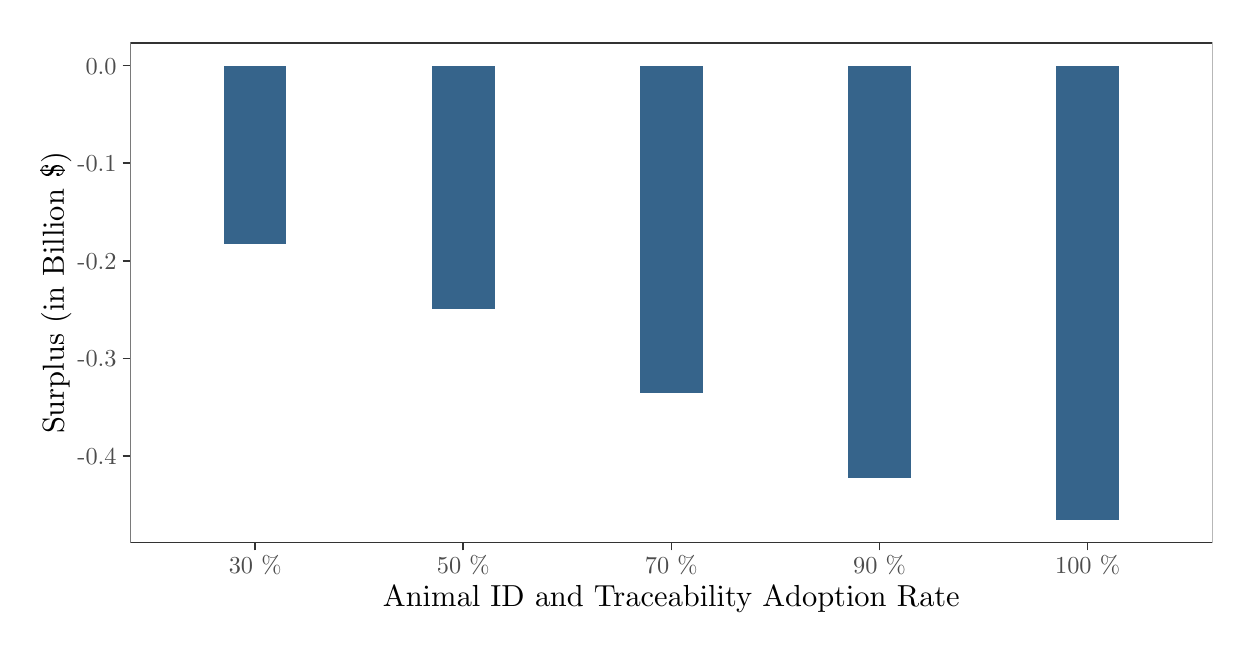
\begin{tikzpicture}[x=1pt,y=1pt]
\definecolor{fillColor}{RGB}{255,255,255}
\path[use as bounding box,fill=fillColor,fill opacity=0.00] (0,0) rectangle (433.62,216.81);
\begin{scope}
\path[clip] (  0.00,  0.00) rectangle (433.62,216.81);
\definecolor{drawColor}{RGB}{255,255,255}
\definecolor{fillColor}{RGB}{255,255,255}

\path[draw=drawColor,line width= 0.6pt,line join=round,line cap=round,fill=fillColor] (  0.00,  0.00) rectangle (433.62,216.81);
\end{scope}
\begin{scope}
\path[clip] ( 37.09, 30.69) rectangle (428.12,211.31);
\definecolor{fillColor}{RGB}{255,255,255}

\path[fill=fillColor] ( 37.09, 30.69) rectangle (428.12,211.31);
\definecolor{fillColor}{RGB}{54,100,139}

\path[fill=fillColor] ( 70.93,138.51) rectangle ( 93.49,203.10);

\path[fill=fillColor] (146.13,115.16) rectangle (168.69,203.10);

\path[fill=fillColor] (221.32, 84.65) rectangle (243.88,203.10);

\path[fill=fillColor] (296.52, 54.13) rectangle (319.08,203.10);

\path[fill=fillColor] (371.72, 38.90) rectangle (394.28,203.10);
\definecolor{drawColor}{gray}{0.20}

\path[draw=drawColor,line width= 0.6pt,line join=round,line cap=round] ( 37.09, 30.69) rectangle (428.12,211.31);
\end{scope}
\begin{scope}
\path[clip] (  0.00,  0.00) rectangle (433.62,216.81);
\definecolor{drawColor}{gray}{0.30}

\node[text=drawColor,anchor=base east,inner sep=0pt, outer sep=0pt, scale=  0.88] at ( 32.14, 58.97) {-0.4};

\node[text=drawColor,anchor=base east,inner sep=0pt, outer sep=0pt, scale=  0.88] at ( 32.14, 94.25) {-0.3};

\node[text=drawColor,anchor=base east,inner sep=0pt, outer sep=0pt, scale=  0.88] at ( 32.14,129.52) {-0.2};

\node[text=drawColor,anchor=base east,inner sep=0pt, outer sep=0pt, scale=  0.88] at ( 32.14,164.79) {-0.1};

\node[text=drawColor,anchor=base east,inner sep=0pt, outer sep=0pt, scale=  0.88] at ( 32.14,200.07) {0.0};
\end{scope}
\begin{scope}
\path[clip] (  0.00,  0.00) rectangle (433.62,216.81);
\definecolor{drawColor}{gray}{0.20}

\path[draw=drawColor,line width= 0.6pt,line join=round] ( 34.34, 62.00) --
	( 37.09, 62.00);

\path[draw=drawColor,line width= 0.6pt,line join=round] ( 34.34, 97.28) --
	( 37.09, 97.28);

\path[draw=drawColor,line width= 0.6pt,line join=round] ( 34.34,132.55) --
	( 37.09,132.55);

\path[draw=drawColor,line width= 0.6pt,line join=round] ( 34.34,167.83) --
	( 37.09,167.83);

\path[draw=drawColor,line width= 0.6pt,line join=round] ( 34.34,203.10) --
	( 37.09,203.10);
\end{scope}
\begin{scope}
\path[clip] (  0.00,  0.00) rectangle (433.62,216.81);
\definecolor{drawColor}{gray}{0.20}

\path[draw=drawColor,line width= 0.6pt,line join=round] ( 82.21, 27.94) --
	( 82.21, 30.69);

\path[draw=drawColor,line width= 0.6pt,line join=round] (157.41, 27.94) --
	(157.41, 30.69);

\path[draw=drawColor,line width= 0.6pt,line join=round] (232.60, 27.94) --
	(232.60, 30.69);

\path[draw=drawColor,line width= 0.6pt,line join=round] (307.80, 27.94) --
	(307.80, 30.69);

\path[draw=drawColor,line width= 0.6pt,line join=round] (383.00, 27.94) --
	(383.00, 30.69);
\end{scope}
\begin{scope}
\path[clip] (  0.00,  0.00) rectangle (433.62,216.81);
\definecolor{drawColor}{gray}{0.30}

\node[text=drawColor,anchor=base,inner sep=0pt, outer sep=0pt, scale=  0.88] at ( 82.21, 19.68) {30 \%};

\node[text=drawColor,anchor=base,inner sep=0pt, outer sep=0pt, scale=  0.88] at (157.41, 19.68) {50 \%};

\node[text=drawColor,anchor=base,inner sep=0pt, outer sep=0pt, scale=  0.88] at (232.60, 19.68) {70 \%};

\node[text=drawColor,anchor=base,inner sep=0pt, outer sep=0pt, scale=  0.88] at (307.80, 19.68) {90 \%};

\node[text=drawColor,anchor=base,inner sep=0pt, outer sep=0pt, scale=  0.88] at (383.00, 19.68) {100 \%};
\end{scope}
\begin{scope}
\path[clip] (  0.00,  0.00) rectangle (433.62,216.81);
\definecolor{drawColor}{RGB}{0,0,0}

\node[text=drawColor,anchor=base,inner sep=0pt, outer sep=0pt, scale=  1.10] at (232.60,  7.64) {Animal ID and Traceability Adoption Rate};
\end{scope}
\begin{scope}
\path[clip] (  0.00,  0.00) rectangle (433.62,216.81);
\definecolor{drawColor}{RGB}{0,0,0}

\node[text=drawColor,rotate= 90.00,anchor=base,inner sep=0pt, outer sep=0pt, scale=  1.10] at ( 13.08,121.00) {Surplus (in Billion \$)};
\end{scope}
\end{tikzpicture}
